\documentclass[paper=a4,fontsize=11pt]{temp} % KOMA-article 
\usepackage{array}

\begin{document}
\sepspace
\begin{minipage}{.15\linewidth}
  % 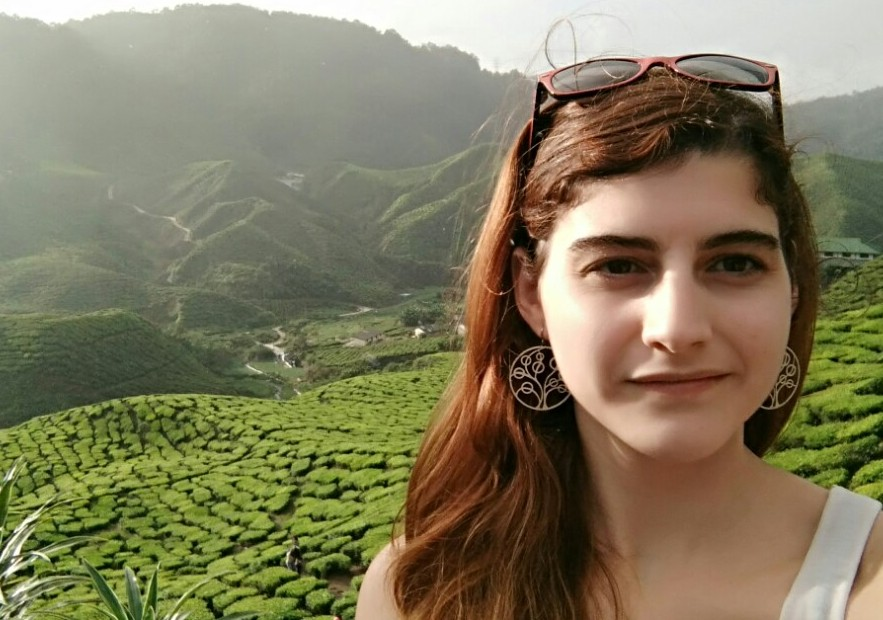
\includegraphics[width=1.4\textwidth]{ana2}
   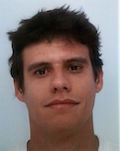
\includegraphics[width=\textwidth]{quim}
\end{minipage}      
\begin{minipage}{0.75\linewidth}
   \MyName{Joaquim Bellmunt Montoya}
   \sepspace
   \noindent
   
   \hfill    
   \begin{tabular}[width=\textwidth]{@{}cl@{}}
   \setlength{\tabcolsep}{12pt}
   \begin{tabular}{>{\centering\arraybackslash}p{.55\textwidth}} \centering \small \textit{Interested in technological innovations that respond to societal demands.\\Pervasive Computation, Internet of Things, and Cloud Computing.} \end{tabular}
   & \setlength{\tabcolsep}{5pt} \begin{tabular}{@{}cl@{}}
    
\includegraphics[height=2ex]{IMG/icons/profile} & Barcelona, Oc 15th 1987  \\
    
\includegraphics[height=2ex]{IMG/icons/mail9} & joaquim.bell@gmail.com  \\
    
\includegraphics[height=2ex]{IMG/icons/telephone1} &(+65) 81193783 \\    
    
\includegraphics[height=2ex]{IMG/icons/social6}  &  quimbell\\    
    
\includegraphics[height=2ex]{IMG/icons/map5}  & Singapore   
   \end{tabular}
 \end{tabular}
   %\hfill yourwebsite.com
   
   %\hfill (+351)93123123123  
 
\end{minipage}


\NewPart{Work experience}{}
\noindent


\workEntry{IPAL (CNRS UMI)}{Jul 2014 - Today}{Research Assistant}{Ph.D. Student at Image and Pervasive Access Lab. I Focus on Semantic Reasoning, Human Condition Computation, Context-Aware Service Delivery and User Interface Plasticity in Ambient Assisted Living deployments for ageing in place and dependent people.} {IMG/ipal}
\sepspace

%\workEntrySmall{Nanyang Techonological University}{Fall 2016}{Teaching Assistant}{Teacher at the Algorithms CE2001 module lab.}{IMG/NTUE}

%\sepspace

\workEntrySmall{KPMG}{Nov 2013 - Apr 2014}{IT Auditor}{Systems \& Process Assurance Auditor for annual audits in several multinational companies.}{IMG/kpmg}

\sepspace

\workEntry{LIRMM}{Mar 2013 - Sep 2013}{Research Intern}{Intern at Laboratoire d'Informatique, Robotique et Micro-Éléctronique de Montpellier. Master thesis Internship in medical robotics field.} {IMG/LIRMM}

\sepspace

\workEntrySmall{Dept. of Signal Theory and Communications}{Feb 2011 - Jan 2012}{Fellow Intern}{Intern at UPC. In charge of computer maintenance and support for all department staff.}{IMG/upc}


%\sepspace

%\workEntrySmall{Centre Municipal de Vela Barcelona}{2008-2011}{Sailing Instructor}{Summer sailing courses for kids of all ages and adults.}{IMG/cmv}


\NewPart{Education}{}
\noindent


\EducationEntry{Phd. at IPAL}{Jul 2014 - Today}{Computer Science Doctoral School I2S, University of Montpelier, France}{Institut Mines-télécom French Ph.D. based on Singapore} {IMG/imt}

\sepspace


\EducationEntry{ICT for Health Specialisation}{Sep 2012 - Sep 2013}{Institut Mines-Télécom, Université Montpellier, École des Mines d'Alès, Montpelier, France}{Bachelor and Master Degree with specialty in Communications.\\9.5/10 qualification for my Thesis, average grade of 7.33/10, order 33/144 and efficiency of 0.94.} {IMG/imt}

\sepspace


\EducationEntry{MSc. Telecommunications Engineering}{Feb 2012 - Sep 2013}{ENS Telecom Bretagne, Brest, France}{Double Master Degree program.} {IMG/Brest}

\sepspace


\EducationEntry{BSc and MSc. Telecommunications Engineering}{Sep 2005 - Jan 2012}{TelecomBCN (ETSETB, UPC Barcelona Tech), Spain}{Bachelor and Master Degree in Telecommunications.} {IMG/logo_telecom_S}


%\sepspace

\NewPart{Skills \& Interests}{}
\hspace{3mm}
\begin{minipage}[t]{0.33\textwidth} 

\begin{tabular}[t]{ l l }
\flag{IMG/flag/es}  & Native Speaker \\
\flag{IMG/flag/cat} & Native Speaker \\
\flag{IMG/flag/fr}  & Bilingual\\%Conversational level \\
\flag{IMG/flag/gb}  & Full competence \\
%Professional Proficiency \\
\end{tabular}

\sepspace

\end{minipage}
%
\begin{minipage}[t]{0.66\textwidth} 

\begin{tabular}[t]{l l}
\softwareb{IMG/soft/computer}  	 &\small \begin{tabular}[t]{@{}l@{}} Semantic Web, Rule-Based engine, RDF, Notation3.\\
JavaScript, Node.js, REST, MQTT, Bash, Android and Ionic.\\
Classification (M.L.), Python, Matlab, R, and Weka.\\
Mac, Windows and Linux OS.\end{tabular} \vspace{.7ex}
\\
\softwareb{IMG/hobbie}  &\small\setlength\extrarowheight{-1ex}\begin{tabular}[t]{@{}p{.8\linewidth}@{}}
Any ball sport, specially Football, and Barça fan. Cinema, traveling, driving.
\end{tabular} \\
\end{tabular}
\end{minipage}

\setlength\extrarowheight{-1ex}
\vspace{1ex}
\begin{tabular}{l l}
%
\softwareb{IMG/people}  &\small  \begin{tabular}[t]{@{}p{.85\linewidth}@{}}
- Founder and Manager of a two football teams in Singapore regrouping European people.\\

- Board member of Telecogresca A.C (http://www.telecogresca.com) in 2011 and 2012. It is a student
association, which organizes a music festival hosting every year more than 10.000 people.\\

- Former Vice-President of the sports student association in my college, CET, Club Esportiu Telecos,
which organises every semester different sportive competitions, such as Football, Basketball or
Volleyball.
\end{tabular} 
\end{tabular}

%
\pagebreak
\sepspace

\NewPart{Publications}{}
\hspace{3mm}
\begin{minipage}{0.04\linewidth}
        \hspace{\linewidth}
		\end{minipage}%  
   \begin{minipage}{0.88\linewidth}
   %\noindent\hangindent=2em\hangafter=1 
    
    - \textbf{Bellmunt, J.}, Tiberghien, T., Mokhtari, M., Aloulou, H., \& Endelin, R. (2015, June). Technical Challenges Towardsan AAL Large Scale Deployment. In International Conference on Smart Homes and Health Telematics (pp.3-14). Springer International Publishing. \textbf{Published}\\
    
    - Aloulou, H., Abdulrazak, B., Endelin, R., Bentes, J., Tiberghien, T., \& \textbf{Bellmunt, J.}, (2016, May). Simplifying Installation and Maintenance of Ambient Intelligent Solutions Toward Large Scale Deployment.International Conference on Smart Homes and Health Telematics, \textbf{Published}.\\
    
   - \textbf{Bellmunt, J.}, Mokhtari, M., Abdulrazak, B., Aloulou, H., \& Kodys, M., (2016, November). Experimental Frailty Model Towards an Adaptable Service Delivery for Aging People. 21th International Conference on Engineering of Complex Computer Systems. \textbf{Presented}\\
   
    - Aloulou, H., Abdulrazak, B., Endelin, R., Kadachi, F., \& \textbf{Bellmunt, J.}, (2016, November). Detecting Inconsistencies in Rule-Based Reasoning for Ambient Intelligence. 21th International Conference on Engineering of Complex Computer Systems. \textbf{Presented}\\
    
    - \textbf{Bellmunt, J.}, Mokhtari, M., Abdulrazak, B, \& Aloulou, H., (2016, June). Agile Framework for Rapid Deployment in Ambient Assisted Living Environments. International Conference on Information Integration and Web-based Applications \& Services. \textbf{Accepted in IIWAS (28-30 Nov 2016).}\\
    
    - Bellmunt, J., Abdulzarak, B., Mokhtari, M., \& Aloulou, H., (2017). Adaptable Computational Model for Frailty Measurement in Ambient Intelligence Environment. BHI-2017 International Conference on Biomedical and Health Informatics 2017. \textbf{Submitted}\\
    
    - Aloulou, H., Abdulrazak, B., Endelin, R., Kadachi, F., \& \textbf{Bellmunt, J.}. (2017). Activity Recognition Enhancement Based on Groundtruth: Introducing Accuracy and Granularity Metrics. IEEE
International Conference on Pervasive Computing and Communications. \textbf{Submitted}.\\

   \end{minipage}        
\sepspace

\NewPart{Honors \& Awards}{}
\hspace{3mm}
\begin{minipage}[t]{0.45\textwidth}
\AwardEntry{IoT Hackathon}{Apr 2015}{First Runner Up  at IoT Hackaton organized by I²R/A*STAR - ETPL - SIAA} {IMG/Logo_of_A-STAR}
\end{minipage}
% \hspace{0.02\textwidth}
% \begin{minipage}[t]{0.45\textwidth}
% \AwardEntry{Obra Social "La Caixa"}{Apr 2015}{Scholarship to cover additional conference and travel expenses during my PhD.} {IMG/lacaixa}
% \end{minipage}

\sepspace

\NewPart{Referees}{}
\hspace{3mm}
\begin{minipage}[t]{0.45\textwidth}
\RefereeEntry{Prof. Mounir Mokhtari}{}{Ph.D. director \\ IPAL Director \\ Professor at Institut Mines-Télécom\\mounir.mokhatri@iipal.cnrs.fr} {pics/limjoohwee}
\end{minipage}
\hspace{0.02\textwidth}
\begin{minipage}[t]{0.45\textwidth}
\RefereeEntry{Prof. Bessam Abdulzarak}{}{Ph.D. Advisor\\ IPAL collaborator\\ University of Sherbrooke (UdeS)\\bessam.abdulrazak@usherbrooke.ca} {pics/ahhwee}
\end{minipage}
 \sepspace
 


%%% References
%%% ------------------------------------------------------------

\end{document}
